\newpage
\section{Simcenter}

CAE(Computer-aided engineering) este un termen pentru a definii un tip de aplicație folosită în domeniul ingineriei pentru
 a rezolva diferite probleme ce țin de arii științifice precum: analiza finita a elementelor (FEA), mecanica fluidelor numerică (CFD), 
 durabilitate materiialelor și optimizare. Acest tip de aplicație este folosit pentru a analiza rezistența și performanța anumitor componente 
 sau ansambluri de componente, eficientizând timpul și materia necesara în întregul proces, in special datorita aspectului digital.
Este folosit în multe domenii precum industria de auto-motive, aviație și aeronautica.\newline

Ariile acoperite de CAE sunt:
\begin{itemize}
\item analiza stresului anumitor componente folosind FEA
\item analiza fluidelor prin CFD
\item cinematica
\item simularea formării unei componente prin turnarea, presarea materiialelor de construcție
\item optimizarea produsului 
\item optimizarea procesului de creare
\end{itemize}

In general sunt trei etape care formează întregul proces de analiza:
\begin{itemize}
    \item pre-procesare: se definește modelul și factorii de mediu 
    \item analiza: proces care este rulat pe o unitate de calculare performanta
    \item post-procesarea: se afișează rezultatele utilizând aplicații de vizualizare
\end{itemize}

Acest ciclu este rulat iterativ de mai multe ori fie manual fie prin aplicații de optimizare.\newline

Aplicațiile CAE sunt folosite foarte des în industria de automotive. Folosirea lor a dat posibilitatea de a 
reduce costul și timpul de producție în timp ce au îmbunătățit siguranța, confortul și durabilitatea vehiculelor produse. 
S-a ajuns în punctul în care se preferă testarea produselor într-un mediu digital decât pe un prototip fizic.\newline

Simcenter Motion este o aplicație software CAE folosită pentru animarea și analizarea mecanismelor cinematice și dinamice în 
legătură cu puncte de design critice, forțe, viteze, accelerații.\newline

Într-o simulare cinematică:
\begin{itemize}
    \item sarcinile externe și forțele de inerție afectează forțele de reacție ale corpurilor dar nu afectează mișcarea
    \item corpurile și legăturile dintre ele sunt rigide
    \item nu există bucșe sau alte elemente care se pot deforma
\end{itemize}

\begin{figure}[H]
    \begin{center}
        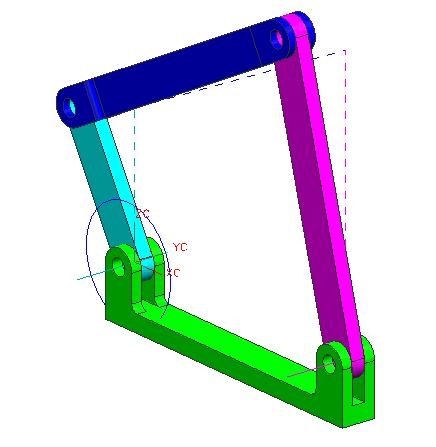
\includegraphics[scale=0.7]{imagini/simcenter/cinematica.png}
        \caption{Model cinematic}
        \label{fig:tabs}
    \end{center}    
\end{figure}

\newpage

Într-o simulare dinamică:
\begin{itemize}
    \item sarcinile externe și forșele pot genera mișcare
    \item există bucșe pentru simularea legăturilor de supunere
    \item există efecte ce țin de forțe de frecare și contact 
    \item se poate rula o analiză de echilibru static în care toate forțele externe și interne sunt în echilibru
\end{itemize}

\begin{figure}[H]
    \begin{center}
        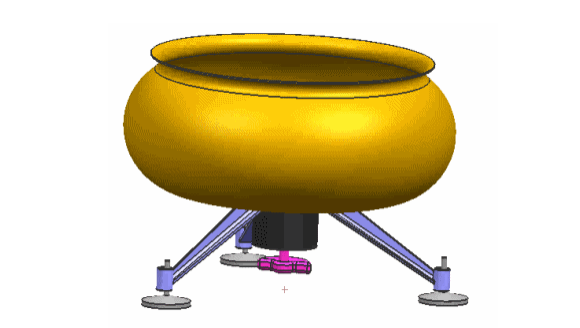
\includegraphics[scale=0.7]{imagini/simcenter/dinamic.png}
        \caption{Model dinamic}
        \label{fig:tabs}
    \end{center}    
\end{figure}

In aplicație un mecanism se definește ca fiind un ansamblu de componente rigide care se mișcă coeziv. 
Pentru a crea un mecanism este necesară:
\begin{itemize}
    \item specificarea corpurilor de mișcare și corpurilor statice
    \item constrângerea mișcării dintre corpuri, prin definirea mișcării unui corp în legătură cu celelalte corpuri. 
    Acestea se crează prin legături dintre corpurile de mișcare.
    \item setarea întregii mișcări ale mecanismului
\end{itemize}

\begin{figure}[H]
    \begin{center}
        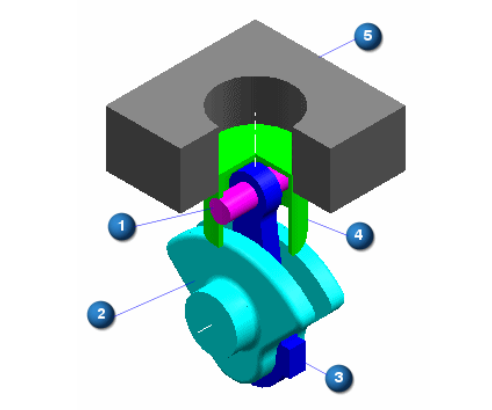
\includegraphics[scale=0.7]{imagini/simcenter/mecanism.png}
        \caption{Model mecanism}
        \label{fig:tabs}
    \end{center}    
\end{figure}

Corpurile de mișcare reprezintă elemente rigide în mecanism. Orice componentă din model ce se poate mișca trebuie 
înclusa într-un corp de mișcare. Un corp de mișcare poate fi reprezentat fie printr-o componentă de asamblare fie 
prin corpuri geometrice simple solide, linii curbe sau puncte. De obicei este mai ușor în procesul de creare a mecanismului sa 
fie definit inițial prin elemente simple precum linii curbe și puncte pentru a verifica un comportament elementar 
ca apoi detaliile sa fie adăugate.\newline

\begin{figure}[H]
    \begin{center}
        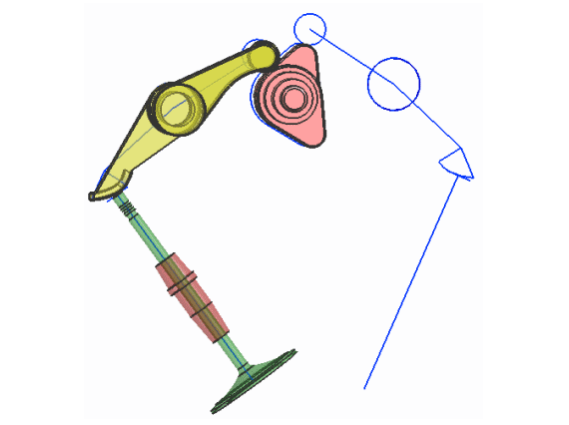
\includegraphics[scale=0.7]{imagini/simcenter/body.png}
        \caption{Model mecanism}
        \label{fig:tabs}
    \end{center}    
\end{figure}

Într-un mecanism un grad de libertate descrie cum un corp de mișcare se poate deplasa relativ la celelalte corpuri. 
Toate gradele de libertate ale unui mecanism descriu toate mișcările independente posibile ale lui. Fară constrângeri 
un corp dintr-un mecanism plutește în spațiu avand șase grade libertate: trei grade de translație (direcția X,  Y sau Z) 
și trei grade de rotație (în jurul axelor X, Y, Z). O îmbinare ale corpurilor constrange unu sau mai multe grade libertate.\newline

Mișcarea unui corp este definită ca fiind mișcarea lui relativa la un corp de baza de care este legat, sau la pământ dacă nu exista.\newline
